\documentclass[12pt]{article}
\usepackage[utf8]{inputenc}
\usepackage{amsmath, amssymb}
\usepackage{xcolor}
\usepackage{geometry}
\usepackage{hyperref}
\usepackage{fancyhdr}
\usepackage{enumitem}
\usepackage{minted} % Code highlighting
\usepackage{booktabs} % Clean tables
\usepackage{tikz}
\usetikzlibrary{shapes, arrows, positioning, automata, calc}

\geometry{margin=1in}
\hypersetup{colorlinks=true, linkcolor=blue, urlcolor=cyan}

\newcommand{\TOPICTITLE}{TCP\: Connection-Oriented Transport}

\pagestyle{fancy}
\fancyhf{}
\fancyhead[L]{\textbf{\TOPICTITLE}}
\fancyhead[R]{\thepage}

% -------------------------------
% Topic Metadata
% -------------------------------
\title{\TOPICTITLE\\\large Study-Ready Notes}
\author{Compiled by Andrew Photinakis}
\date{\today}

\setlength{\headheight}{15pt}

\begin{document}
\maketitle
\tableofcontents
\newpage

% This LaTeX file should be saved at: computer_networks/transport_layer/tcp_connection_oriented_transport.tex

\section{TCP Overview and Key Characteristics}

\begin{itemize}
    \item \textbf{Point-to-point}: One sender, one receiver
    \item \textbf{Reliable, in-order byte stream}: No "message boundaries"
    \item \textbf{Full duplex data}: Bi-directional data flow in same connection
    \item \textbf{MSS}: Maximum Segment Size
    \item \textbf{Cumulative ACKs}: Acknowledgment mechanism
    \item \textbf{Pipelining}: TCP congestion and flow control set window size
    \item \textbf{Connection-oriented}: Handshaking initializes sender/receiver state
    \item \textbf{Flow controlled}: Sender will not overwhelm receiver
\end{itemize}

\textcolor{blue}{[Summary: TCP provides reliable, connection-oriented, full-duplex communication with flow control and congestion control mechanisms to ensure efficient and orderly data transfer between two endpoints.]}

\section{TCP Segment Structure}

\subsection{Segment Format}
\begin{figure}[h]
    \centering
    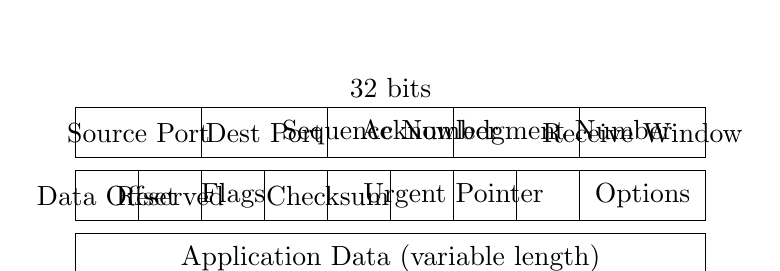
\begin{tikzpicture}[scale=0.8]
        \draw (0,0) rectangle (10,0.8);
        \foreach \x in {0,2,4,6,8,10} {
                \draw (\x,0) -- (\x,0.8);
            }

        \node at (1,0.4) {Source Port};
        \node at (3,0.4) {Dest Port};
        \node at (5,0.4) {Sequence Number};
        \node at (7,0.4) {Acknowledgment Number};
        \node at (9,0.4) {Receive Window};

        % Second row
        \draw (0,-1) rectangle (10,-0.2);
        \foreach \x in {0,1,2,3,4,5,6,7,8,10} {
                \draw (\x,-1) -- (\x,-0.2);
            }

        \node at (0.5,-0.6) {Data Offset};
        \node at (1.5,-0.6) {Reserved};
        \node at (2.5,-0.6) {Flags};
        \node at (4,-0.6) {Checksum};
        \node at (6,-0.6) {Urgent Pointer};
        \node at (9,-0.6) {Options};

        % Application data
        \draw (0,-2) rectangle (10,-1.2);
        \node at (5,-1.6) {Application Data (variable length)};

        \node[above] at (5,0.8) {32 bits};
    \end{tikzpicture}
    \caption{TCP segment structure showing key fields and their organization}
    \label{fig:tcp_segment}
\end{figure}

\subsection{Key Field Descriptions}
\begin{itemize}
    \item \textbf{Sequence Number}: Byte stream number of first byte in segment's data
    \item \textbf{Acknowledgment Number}: Sequence number of next expected byte (when ACK flag set)
    \item \textbf{Receive Window}: Number of bytes receiver is willing to accept (flow control)
    \item \textbf{Flags}: Control bits (SYN, ACK, FIN, RST, PSH, URG)
    \item \textbf{Checksum}: Internet checksum for error detection
\end{itemize}

\textcolor{orange}{[Mnemonic: "SP DS AN RW" - Source Port, Destination Port, Ack Number, Receive Window - key TCP header fields.]}

\section{TCP Sequence Numbers and Acknowledgments}

\subsection{Sequence Number Space}
\begin{itemize}
    \item Sequence numbers count \textbf{bytes} in the byte stream, not segments
    \item Each byte of data is assigned a sequence number
    \item Initial sequence numbers chosen during connection establishment
\end{itemize}

\subsection{Acknowledgment Mechanism}
\begin{itemize}
    \item \textbf{Cumulative ACKs}: ACK(n) acknowledges all bytes up to sequence number n-1
    \item ACK number indicates the \textbf{next expected byte}
    \item Out-of-order segment handling is implementation-dependent
\end{itemize}

\begin{figure}[h]
    \centering
    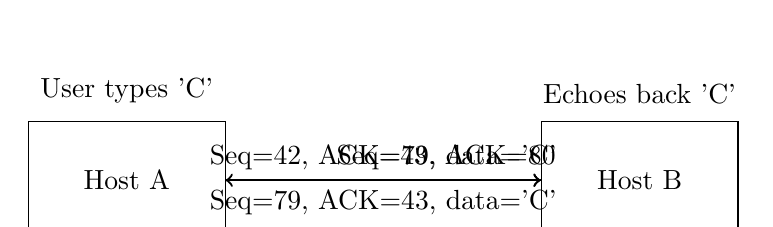
\begin{tikzpicture}[
            node distance=2cm,
            host/.style={rectangle, draw, minimum width=2.5cm, minimum height=1.5cm}
        ]
        \node[host] (hostA) {Host A};
        \node[host, right=4cm of hostA] (hostB) {Host B};

        % Data flow
        \draw[->, thick] (hostA.east) -- node[above] {Seq=42, ACK=79, data='C'} (hostB.west);
        \draw[->, thick] (hostB.west) -- node[below] {Seq=79, ACK=43, data='C'} (hostA.east);
        \draw[->, thick] (hostA.east) -- node[above, pos=0.7] {Seq=43, ACK=80} (hostB.west);

        % Labels
        \node[above=0.1cm of hostA] {User types 'C'};
        \node[above=0.1cm of hostB] {Echoes back 'C'};

    \end{tikzpicture}
    \caption{TCP sequence number exchange in telnet scenario}
    \label{fig:tcp_sequence_example}
\end{figure}

\section{TCP Round Trip Time and Timeout}

\subsection{RTT Estimation Challenge}
\begin{itemize}
    \item Timeout must be longer than RTT, but RTT varies
    \item \textbf{Too short}: Premature timeout, unnecessary retransmissions
    \item \textbf{Too long}: Slow reaction to segment loss
\end{itemize}

\subsection{Exponential Weighted Moving Average (EWMA)}
\[
    \text{EstimatedRTT} = (1 - \alpha) \times \text{EstimatedRTT} + \alpha \times \text{SampleRTT}
\]
Where:
\begin{itemize}
    \item $\text{SampleRTT}$: Measured time from segment transmission to ACK receipt
    \item $\alpha$: Smoothing factor (typically 0.125)
    \item Influence of past samples decreases exponentially
\end{itemize}

\subsection{Timeout Interval Calculation}
\[
    \text{TimeoutInterval} = \text{EstimatedRTT} + 4 \times \text{DevRTT}
\]
\[
    \text{DevRTT} = (1 - \beta) \times \text{DevRTT} + \beta \times |\text{SampleRTT} - \text{EstimatedRTT}|
\]
Where $\beta$ is typically 0.25.

\begin{figure}[h]
    \centering
    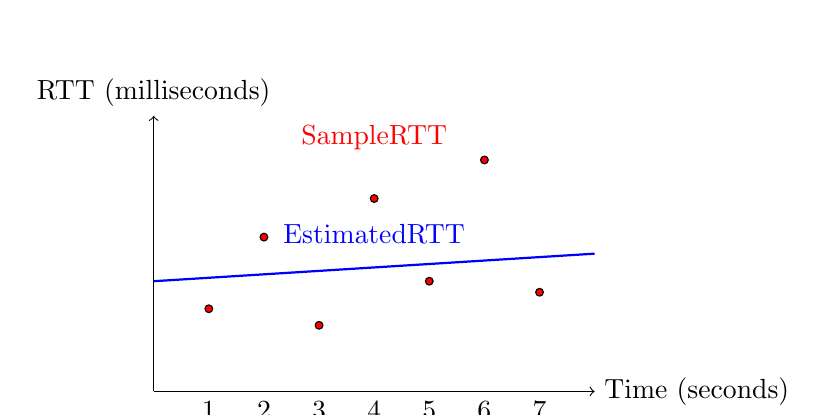
\begin{tikzpicture}[scale=0.7]
        \draw[->] (0,0) -- (8,0) node[right] {Time (seconds)};
        \draw[->] (0,0) -- (0,5) node[above] {RTT (milliseconds)};

        % Sample data points
        \foreach \x/\y in {1/1.5, 2/2.8, 3/1.2, 4/3.5, 5/2.0, 6/4.2, 7/1.8} {
                \draw[fill=red] (\x,\y) circle (2pt);
                \node[below] at (\x,0) {\x};
            }

        % Estimated RTT line
        \draw[thick, blue] (0,2) -- (8,2.5);

        \node[above, red] at (4,4.2) {SampleRTT};
        \node[above, blue] at (4,2.5) {EstimatedRTT};

    \end{tikzpicture}
    \caption{RTT measurement and estimation showing SampleRTT variability and smoothed EstimatedRTT}
    \label{fig:rtt_estimation}
\end{figure}

\textcolor{blue}{[Summary: TCP uses exponential weighted moving averages to estimate RTT and its deviation, setting timeout intervals that balance quick loss detection with avoiding premature timeouts.]}

\section{TCP Sender and Receiver Operations}

\subsection{TCP Sender Events}
\begin{itemize}
    \item \textbf{Data received from application}:
          \begin{itemize}
              \item Create segment with sequence number
              \item Sequence number is byte-stream number of first data byte
              \item Start timer if not already running
          \end{itemize}
    \item \textbf{Timeout}:
          \begin{itemize}
              \item Retransmit segment that caused timeout
              \item Restart timer
          \end{itemize}
    \item \textbf{ACK received}:
          \begin{itemize}
              \item If ACK acknowledges previously unACKed segments
              \item Update what is known to be ACKed
              \item Start timer if there are still unACKed segments
          \end{itemize}
\end{itemize}

\subsection{TCP Sender Algorithm (Simplified)}
\begin{minted}{python}
NextSeqNum = InitialSeqNum
SendBase = InitialSeqNum

while True:
    wait for event
    
    if ACK received with ACK field value y:
        if y > SendBase:
            SendBase = y
            if there are not-yet-acked segments:
                start timer
            else:
                stop timer
                
    if data received from application:
        create segment with seq \# = NextSeqNum
        pass segment to IP
        NextSeqNum = NextSeqNum + length(data)
        if timer not running:
            start timer
            
    if timeout:
        retransmit not-yet-acked segment with smallest seq \#
        start timer
\end{minted}


\section{TCP Retransmission Scenarios}

\subsection{Normal Operation}
\begin{itemize}
    \item Segments transmitted and acknowledged in order
    \item Cumulative ACKs cover all bytes up to acknowledged sequence number
\end{itemize}

\subsection{Lost ACK Scenario}
\begin{itemize}
    \item ACK is lost in transit
    \item Subsequent cumulative ACK covers for earlier lost ACK
    \item No retransmission needed if later ACK arrives
\end{itemize}

\subsection{Premature Timeout}
\begin{itemize}
    \item Timer expires before ACK arrives (ACK is delayed)
    \item Sender retransmits segment
    \item Receiver receives duplicate, uses sequence numbers to detect and discard
\end{itemize}

\subsection{TCP Fast Retransmit}
\begin{itemize}
    \item \textbf{Triple duplicate ACKs}: Receiving 3 ACKs for same data
    \item Indicates segments received after a missing segment
    \item Lost segment is likely, so retransmit without waiting for timeout
    \item More responsive than timeout-based retransmission
\end{itemize}

\begin{figure}[h]
    \centering
    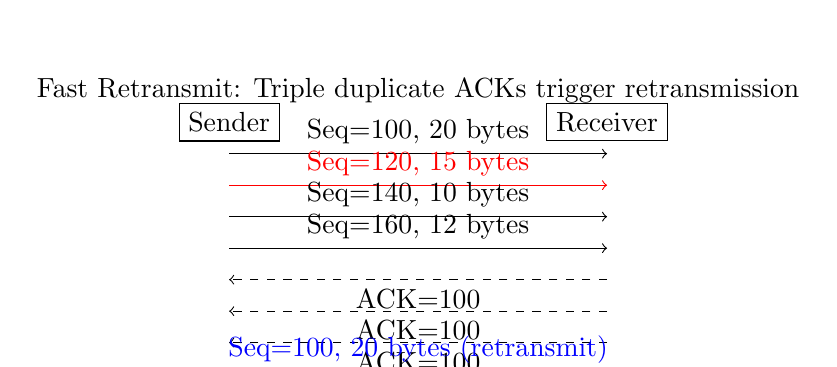
\begin{tikzpicture}[scale=0.8]
        \node[draw, rectangle] (sender) at (0,2) {Sender};
        \node[draw, rectangle] (receiver) at (6,2) {Receiver};

        % Fast retransmit scenario
        \draw[->] (0,1.5) -- node[above] {Seq=100, 20 bytes} (6,1.5);
        \draw[->, red] (0,1.0) -- node[above, sloped] {Seq=120, 15 bytes} (6,1.0);
        \draw[->] (0,0.5) -- node[above] {Seq=140, 10 bytes} (6,0.5);
        \draw[->] (0,0.0) -- node[above] {Seq=160, 12 bytes} (6,0.0);

        % Duplicate ACKs
        \draw[->, dashed] (6,-0.5) -- node[below] {ACK=100} (0,-0.5);
        \draw[->, dashed] (6,-1.0) -- node[below] {ACK=100} (0,-1.0);
        \draw[->, dashed] (6,-1.5) -- node[below] {ACK=100} (0,-1.5);

        % Retransmission
        \draw[->, thick, blue] (0,-2.0) -- node[above] {Seq=100, 20 bytes (retransmit)} (6,-2.0);

        \node at (3,2.5) {Fast Retransmit: Triple duplicate ACKs trigger retransmission};

    \end{tikzpicture}
    \caption{TCP fast retransmit mechanism triggered by triple duplicate ACKs}
    \label{fig:fast_retransmit}
\end{figure}

\textcolor{teal}{[Concept Map: TCP Reliability → Sequence numbers (byte counting) + Cumulative ACKs (efficiency) + Timers (loss detection) + Fast retransmit (quick recovery) = Complete reliability over unreliable networks.]}

\section{TCP Flow Control}

\subsection{Flow Control Problem}
\begin{itemize}
    \item Network layer may deliver data faster than application removes it from socket buffers
    \item Without control, receiver buffers would overflow
    \item Need mechanism to prevent sender from overwhelming receiver
\end{itemize}

\subsection{Receive Window Mechanism}
\begin{itemize}
    \item TCP receiver advertises free buffer space in \textbf{rwnd} field
    \item \textbf{RevBuffer} size set via socket options (typically 4096 bytes)
    \item Many operating systems auto-adjust buffer size
    \item Sender limits unACKed ("in-flight") data to received rwnd value
\end{itemize}

\begin{figure}[h]
    \centering
    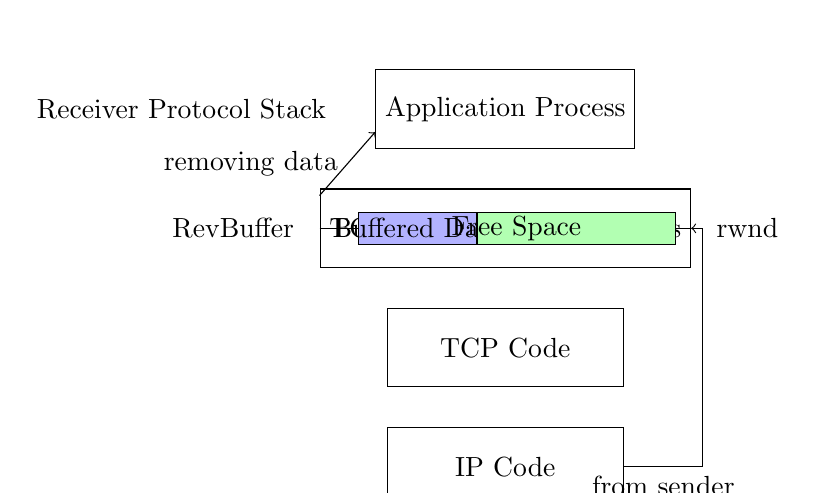
\begin{tikzpicture}[
            node distance=1.5cm,
            box/.style={rectangle, draw, minimum width=3cm, minimum height=1cm}
        ]
        \node[box] (app) {Application Process};
        \node[box, below=0.5cm of app] (buffer) {TCP Socket Receiver Buffers};
        \node[box, below=0.5cm of buffer] (tcp) {TCP Code};
        \node[box, below=0.5cm of tcp] (ip) {IP Code};

        % Buffer details
        \draw (buffer.west) -- (buffer.east);
        \node[left=0.2cm of buffer] {RevBuffer};
        \draw[fill=blue!30] ($(buffer.west)+(0.5,0.2)$) rectangle ($(buffer.west)+(2,-0.2)$);
        \node at ($(buffer.west)+(1.25,0)$) {Buffered Data};
        \draw[fill=green!30] ($(buffer.west)+(2,0.2)$) rectangle ($(buffer.east)+(-0.2,-0.2)$);
        \node at ($(buffer.west)+(2.5,0)$) {Free Space};

        \node[right=0.2cm of buffer] {rwnd};

        % Data flow
        \draw[->] (ip.east) -- node[below] {from sender} ++(1,0) |- (buffer.east);
        \draw[->] (buffer.170) -- node[left] {removing data} (app.-170);

        \node[left=0.5cm of app] {Receiver Protocol Stack};

    \end{tikzpicture}
    \caption{TCP flow control: receiver advertises free buffer space via rwnd field}
    \label{fig:tcp_flow_control}
\end{figure}

\section{TCP Connection Management}

\subsection{Connection Establishment Need}
\begin{itemize}
    \item Agree to establish connection (mutual agreement)
    \item Agree on connection parameters (initial sequence numbers)
    \item Initialize connection state at both ends
\end{itemize}

\subsection{Two-Way Handshake Problems}
\begin{itemize}
    \item \textbf{Half-open connections}: Client terminates, server doesn't know
    \item \textbf{Duplicate data acceptance}: Delayed retransmissions accepted as new data
    \item \textbf{Message reordering}: Cannot handle network reordering properly
\end{itemize}

\subsection{TCP Three-Way Handshake}
\begin{figure}[h]
    \centering
    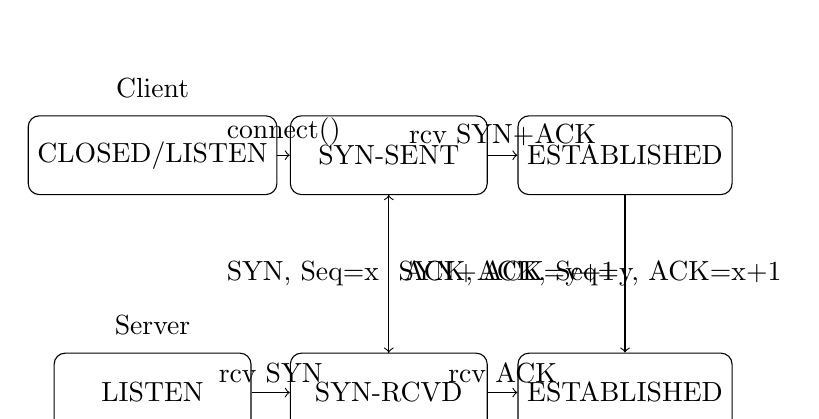
\begin{tikzpicture}[
            node distance=3cm,
            state/.style={rectangle, draw, rounded corners, minimum width=2.5cm, minimum height=1cm}
        ]
        \node[state] (client_listen) {CLOSED/LISTEN};
        \node[state, right of=client_listen] (client_syn_sent) {SYN-SENT};
        \node[state, right of=client_syn_sent] (client_estab) {ESTABLISHED};

        \node[state, below=2cm of client_listen] (server_listen) {LISTEN};
        \node[state, right of=server_listen] (server_syn_rcvd) {SYN-RCVD};
        \node[state, right of=server_syn_rcvd] (server_estab) {ESTABLISHED};

        % Handshake messages
        \draw[->] (client_syn_sent) -- node[left] {SYN, Seq=x} (server_syn_rcvd);
        \draw[->] (server_syn_rcvd) -- node[right] {SYN+ACK, Seq=y, ACK=x+1} (client_syn_sent);
        \draw[->] (client_estab) -- node[left] {ACK, ACK=y+1} (server_estab);

        % State transitions
        \draw[->] (client_listen) -- node[above] {connect()} (client_syn_sent);
        \draw[->] (client_syn_sent) -- node[above] {rcv SYN+ACK} (client_estab);

        \draw[->] (server_listen) -- node[above] {rcv SYN} (server_syn_rcvd);
        \draw[->] (server_syn_rcvd) -- node[above] {rcv ACK} (server_estab);

        \node[above=0.1cm of client_listen] {Client};
        \node[above=0.1cm of server_listen] {Server};

    \end{tikzpicture}
    \caption{TCP three-way handshake: state transitions and message exchange}
    \label{fig:three_way_handshake}
\end{figure}

\subsection{Human Analogy: Rock Climbing}
\begin{enumerate}
    \item \textbf{"On belay?"} (SYN): Climber asks if belayer is ready
    \item \textbf{"Belay on."} (SYN-ACK): Belayer confirms readiness
    \item \textbf{"Climbing."} (ACK): Climber acknowledges and begins
\end{enumerate}

\subsection{Connection Termination}
\begin{itemize}
    \item Client and server each close their side of connection
    \item Send TCP segment with FIN bit = 1
    \item Respond to received FIN with ACK
    \item FIN and ACK can be combined
    \item Simultaneous FIN exchanges handled gracefully
\end{itemize}

\begin{table}[h]
    \centering
    \begin{tabular}{p{0.3\textwidth}p{0.3\textwidth}p{0.3\textwidth}}
        \toprule
        \textbf{2-Way Handshake}            & \textbf{3-Way Handshake}       & \textbf{Advantage}               \\
        \midrule
        Vulnerable to half-open connections & Prevents half-open connections & Complete state synchronization   \\
        Duplicate data acceptance           & Sequence number validation     & Prevents old duplicate confusion \\
        Simple but unreliable               & Robust and reliable            & Handles network variability      \\
        Not used in practice                & TCP standard                   & Industry standard                \\
        \bottomrule
    \end{tabular}
    \caption{Comparison of 2-way vs 3-way handshake}
    \label{tab:handshake_comparison}
\end{table}

\textcolor{blue}{[Summary: TCP uses a three-way handshake for reliable connection establishment, solving problems of half-open connections and duplicate data that plague simpler two-way handshakes, with clear state synchronization.]}

\section{Study Aids and Exam Preparation}

\subsection{Key Concepts to Master}
\begin{itemize}
    \item Understand TCP segment structure and field purposes
    \item Be able to calculate and interpret sequence numbers and ACKs
    \item Know the RTT estimation formulas and timeout calculation
    \item Explain TCP flow control mechanism and rwnd usage
    \item Trace through three-way handshake and connection termination
    \item Compare and contrast different retransmission scenarios
\end{itemize}

\subsection{Practice Questions}
\begin{enumerate}
    \item \textbf{Calculate TCP timeout} given the following: EstimatedRTT = 200ms, DevRTT = 50ms, $\alpha = 0.125$, $\beta = 0.25$. If the next SampleRTT is 180ms, what is the new TimeoutInterval?

    \item \textbf{Trace the three-way handshake} between client (starting seq=1000) and server (starting seq=5000). Show the sequence and acknowledgment numbers in each segment.

    \item Explain how \textbf{TCP flow control} prevents buffer overflow at the receiver. What happens if the application stops reading data from the socket?

    \item Compare \textbf{timeout-based retransmission} vs \textbf{fast retransmit}. Under what conditions is each mechanism triggered, and which is more efficient?

    \item A TCP sender has SendBase = 2000 and NextSeqNum = 2500. The receiver's window is 1000 bytes. How much data can the sender transmit without receiving new ACKs? What happens when rwnd becomes 0?
\end{enumerate}

\textcolor{orange}{[Mnemonic: "SYN SYN-ACK ACK" - The three steps of TCP handshake, easy to remember for connection establishment.]}

\section{Summary}

\begin{itemize}
    \item TCP provides reliable, connection-oriented byte stream service
    \item Sequence numbers count bytes, not segments, enabling accurate tracking
    \item Cumulative ACKs provide efficient acknowledgment mechanism
    \item Adaptive timeout calculation using EWMA of RTT and its deviation
    \item Flow control prevents receiver buffer overflow through rwnd advertising
    \item Three-way handshake ensures reliable connection establishment
    \item Fast retransmit provides quick recovery from segment loss
    \item Connection management handles both establishment and termination gracefully
\end{itemize}

\section{References}
\begin{itemize}
    \item Kurose, J.F., \& Ross, K.W. (2020). \textit{Computer Networking: A Top-Down Approach (8th ed.)}. Pearson.
    \item RFC 5681: TCP Congestion Control
    \item RFC 793: Transmission Control Protocol
    \item Course: COMPSCI 453 Computer Networks, University of Massachusetts
    \item Professor: Jim Kurose, College of Information and Computer Sciences
    \item Textbook website: http://gala.cs.umass.edu/kurose\_ross
    \item Interactive exercises: http://gaia.cs.umass.edu/kurose\_ross/interactive/
\end{itemize}

\end{document}